\subsection{Self-adapting techniques}
\label{sec:selfadapting}

A self-aware adaptive computing system is an active system where the hardware, the applications and the operating system have to be seen as an unique entity that can autonomously adapt itself to achieve the best performance. \cite{selfaware} presents a general overview of the hardware and software architecture components of a self-aware computing system as can be seen in figure \ref{fig:selfaware}. Cognitive hardware mechanisms available in the underlying hardware \emph{observe} and \emph{affect} the exectution. A limited amount of scenarios can be pre-configured, but the learning and decision engines are needed to determine the appropriate actions based on the observations. 

% -- Plaatje self-aware hardware and software architecture---------------------------
\begin{figure}[htb]%
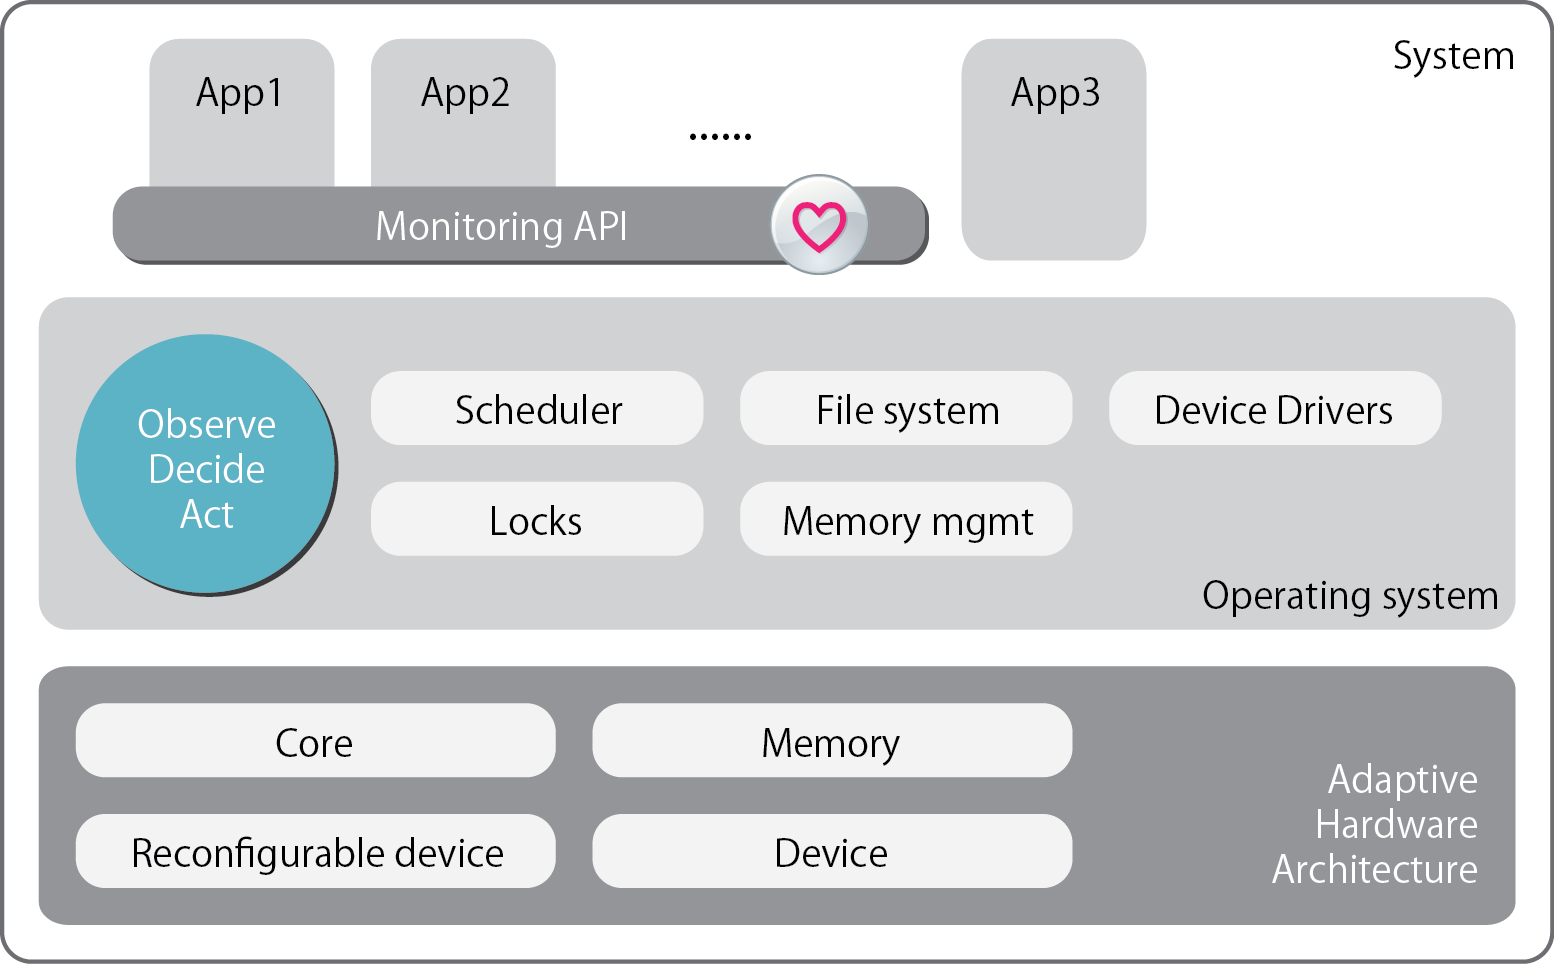
\includegraphics[width=\columnwidth]{Pictures/self-aware.PNG}%
\caption{Overview of the proposed self-aware adaptive FPGA-based computing system presented in \cite{selfaware}}%
\label{fig:selfaware}%
\end{figure}
%------------------------------------------------------------------------------------------------

A fundamental part of a self-aware adaptive computing system is the ability to switch between implementations of the same functionality while the system is running. A control system has to be developed as an actuator in the oberserve-decide-act loop. The \emph{hot-swap mechanism} is a popular tool to inplement self-configuration and self-optimization. It provides the ability of switching among different implementations of the same functionality in a transparent fashion. However state quiescence and state translation are two big issues when using this mechanism and need a framework solution to be reliable. \cite{self-aware} presents a three phase hot-swap that includes a transfer phase in which new requests are blocked to reach a quiescent state to solve this. This approach is solely based on data structures to decouple the data from the implementations.

Other works present \emph{Partial Dynamic Reconfiguration (PDR)} \cite{reconfigurable} to reduce the amount of overhead introduced by reconfiguration. Hardware portions can adapt over time to cope with new requirements creating an adaptive system. If the application can be partitioned into different phases, PDR can configure the modules one after another to keep area requirements lower than having all functionalities loaded at the same time. PDR can be seen as a trade-off between the speed of hardware and the flexibility of software.  